% Backup slides for the presentation, kept out of the main deck.
% Build from this folder:   latexmk -pdf backup.tex

% Shared styling for slides.tex and backup.tex.

\documentclass[aspectratio=169,11pt]{beamer}

\usepackage[T1]{fontenc}
\usepackage{lmodern}
\usepackage{amsmath,amssymb}
\usepackage{booktabs}
\usepackage{tikz}
\usetikzlibrary{arrows.meta,positioning,fit}

\graphicspath{{figures/}{../results/figures/}}

% ------------------------------------------------------------------ appearance
\definecolor{navy}{RGB}{23,50,94}
\definecolor{accent}{RGB}{31,119,180}
\definecolor{good}{RGB}{44,160,44}
\definecolor{warn}{RGB}{214,39,40}
\definecolor{soft}{RGB}{240,244,250}
\setbeamercolor{frametitle}{fg=navy}
\setbeamercolor{title}{fg=navy}
\setbeamercolor{structure}{fg=accent}
\setbeamercolor{block title}{bg=navy,fg=white}
\setbeamercolor{block body}{bg=soft}
\setbeamerfont{frametitle}{series=\bfseries,size=\large}
\setbeamertemplate{navigation symbols}{}
\setbeamertemplate{itemize items}[circle]
\setbeamertemplate{blocks}[rounded][shadow=false]
\setbeamertemplate{footline}{%
  \hfill\usebeamercolor[fg]{structure}\scriptsize\insertframenumber\,/\,\inserttotalframenumber\hspace{1em}\vspace{0.6em}}
\AtBeginSection[]{%
  \begin{frame}[plain,noframenumbering]
    \centering\vfill
    {\Large\bfseries\color{navy}\insertsectionnumber.\ \insertsection}\par\vfill
  \end{frame}}

\newcommand{\E}{\mathbb{E}}
\newcommand{\hl}[1]{\textcolor{accent}{\textbf{#1}}}
\newcommand{\ucvar}{\operatorname{U\text{-}CVaR}}
\newcommand{\bigstat}[2]{%
  \begin{minipage}[t]{\linewidth}\centering
    {\LARGE\bfseries\color{navy}#1}\par\vspace{0.3em}
    {\footnotesize #2\par}
  \end{minipage}}


\begin{document}

\begin{frame}{Backup: the lineups each strategy chose}
  \centering\footnotesize
  \begin{tabular}{@{}lrrp{0.5\textwidth}@{}}
    \toprule
    Strategy & Proj. & Own. & Players \\
    \midrule
    B1 Max projection & 102.7 & 21\,\% & TM1 TE1, TM2 RB1, TM3 QB1, TM3 RB1, TM3 WR4, TM4 WR1, TM6 WR2, TM6 DST, TM8 TE1 \\
    B2 Max proj.\ + stack (= S1) & 102.4 & 24\,\% & TM1 TE1, TM2 RB1, TM2 DST, TM3 QB1, TM3 WR1, TM3 WR4, TM4 RB2, TM4 WR1, TM8 TE1 \\
    S2 field-aware, $\alpha = 0.99$ (= S3) & 85.7 & 9\,\% & TM1 QB1, TM1 RB1, TM1 WR1, TM1 WR3, TM1 TE1, TM3 WR4, TM3 DST, TM6 TE2, TM8 RB2 \\
    S2-CV field-aware, $\alpha = 0.975$ & 91.9 & 13\,\% & TM2 QB1, TM2 RB1, TM2 WR1, TM1 WR1, TM3 WR4, TM6 RB2, TM6 DST, TM8 TE1, TM8 TE2 \\
    \bottomrule
  \end{tabular}
  \vspace{0.8em}
  \begin{itemize}
    \item ``Own.'' is the average field ownership of the lineup's nine players
    \item S3 (maximize simulated expected payout directly) chose the same lineup as S2
    \item S2-CV: TM2's QB, RB1 and WR1 with TM1's WR1 is a game stack with a ``bring-back''
  \end{itemize}
\end{frame}

\begin{frame}{Backup: full out-of-sample results (2,000 contests)}
  \centering\footnotesize
  \begin{tabular}{@{}lrrrrr@{}}
    \toprule
    Strategy & ROI & 95\,\% CI & Cash & Top 1\,\% & Top 0.1\,\% \\
    \midrule
    Typical field lineup & $-15.9\,\%$ & $[-19.0, -12.8]$ & 19.9\,\% & 1.01\,\% & 0.10\,\% \\
    B1 Max projection & $+51.2\,\%$ & $[+22.3, +80.1]$ & 41.3\,\% & 2.00\,\% & 0.15\,\% \\
    B2 Max proj.\ + stack & $+41.1\,\%$ & $[+22.2, +60.0]$ & 40.0\,\% & 2.00\,\% & 0.20\,\% \\
    S1 U-CVaR (points) & $+41.1\,\%$ & $[+22.2, +60.0]$ & 40.0\,\% & 2.00\,\% & 0.20\,\% \\
    S2, $\alpha = 0.99$ & $-15.6\,\%$ & $[-44.0, +12.9]$ & 16.8\,\% & 1.70\,\% & 0.15\,\% \\
    S2-CV, $\alpha = 0.975$ & $+146.4\,\%$ & $[+18.8, +274.0]$ & 25.5\,\% & 2.95\,\% & 0.50\,\% \\
    \bottomrule
  \end{tabular}
  \vspace{0.8em}
  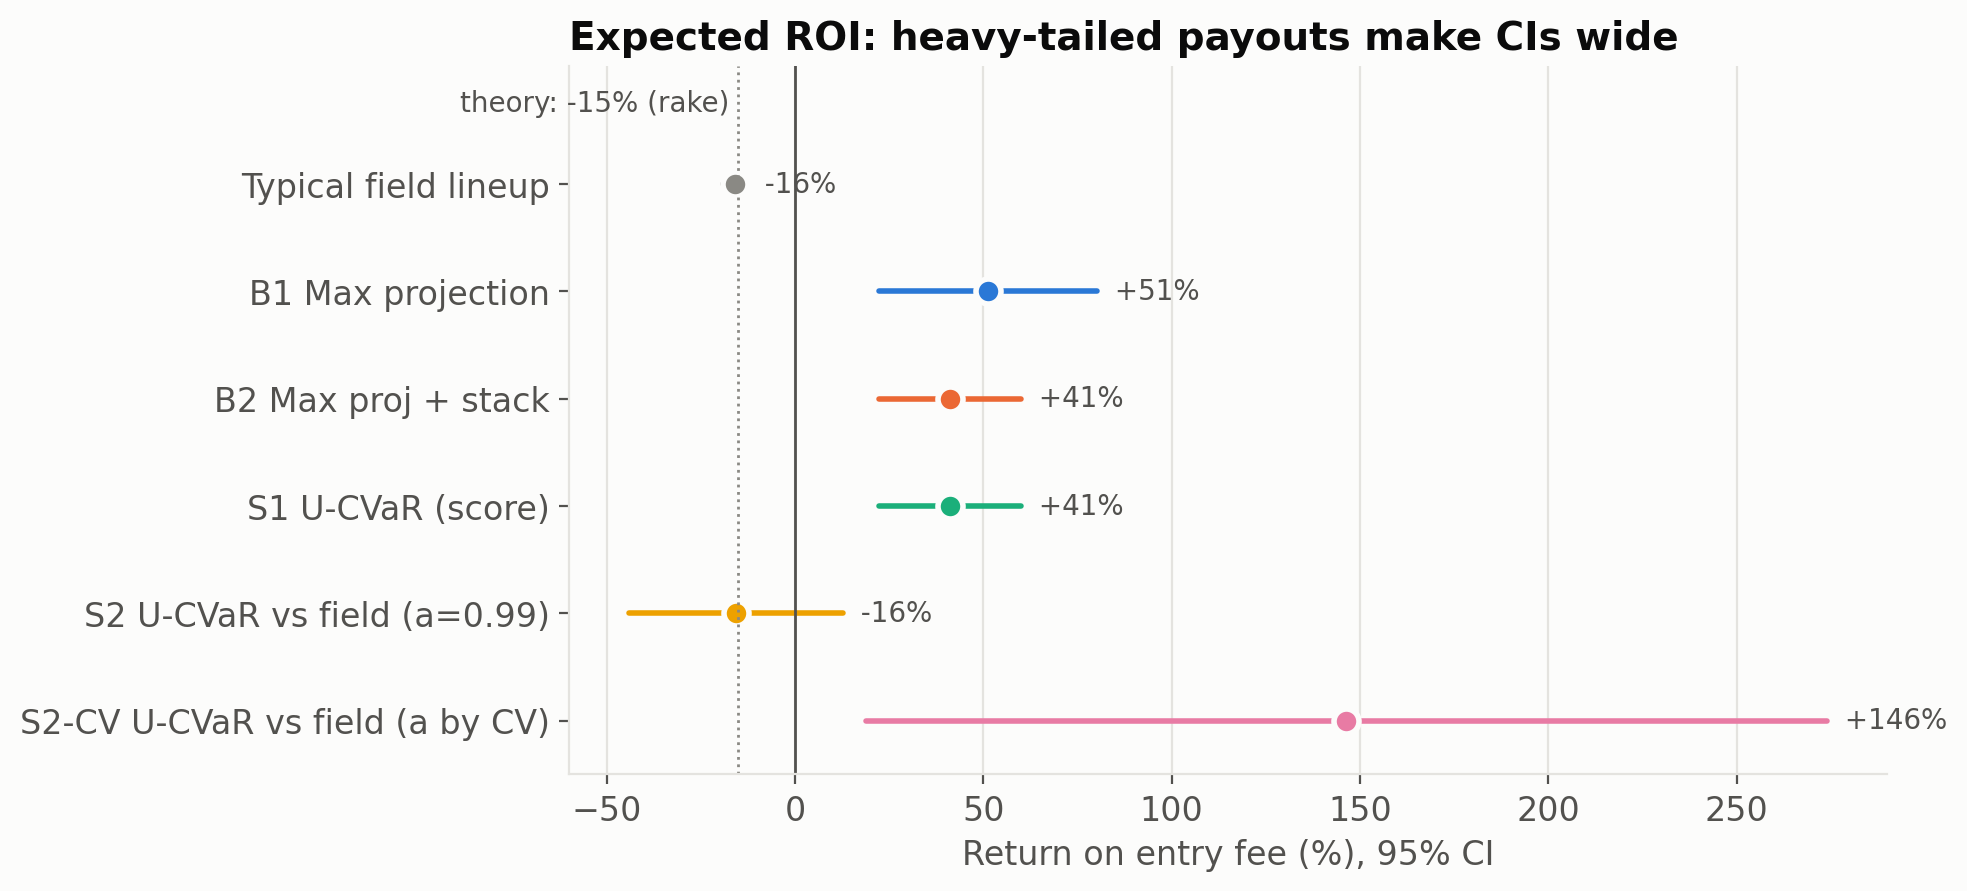
\includegraphics[width=0.5\textwidth]{results_roi}
\end{frame}

\begin{frame}{Backup: choosing $\alpha$ by validation}
  \begin{columns}[c]
    \begin{column}{0.48\textwidth}
      Selection data: 50 fields $\times$ 100 outcome draws.
      \begin{enumerate}
        \item Pick a lineup by field-aware U-CVaR$_\alpha$ on fields 1--25
        \item Score that pick by mean simulated payout on fields 26--50
        \item Keep the best $\alpha$; re-select on all 50 fields
      \end{enumerate}
      The 2{,}000 test contests are never used.
    \end{column}
    \begin{column}{0.48\textwidth}
      \centering
      \begin{tabular}{@{}rr@{}}
        \toprule
        $\alpha$ & Validation payout per \$1 \\
        \midrule
        0.900 & 1.42 \\
        0.950 & 1.43 \\
        \textbf{0.975} & \textbf{3.27} \\
        0.990 & 1.53 \\
        \bottomrule
      \end{tabular}
    \end{column}
  \end{columns}
\end{frame}

\begin{frame}{Backup: the payout table and a single contest}
  \begin{columns}[c]
    \begin{column}{0.49\textwidth}
      \centering
      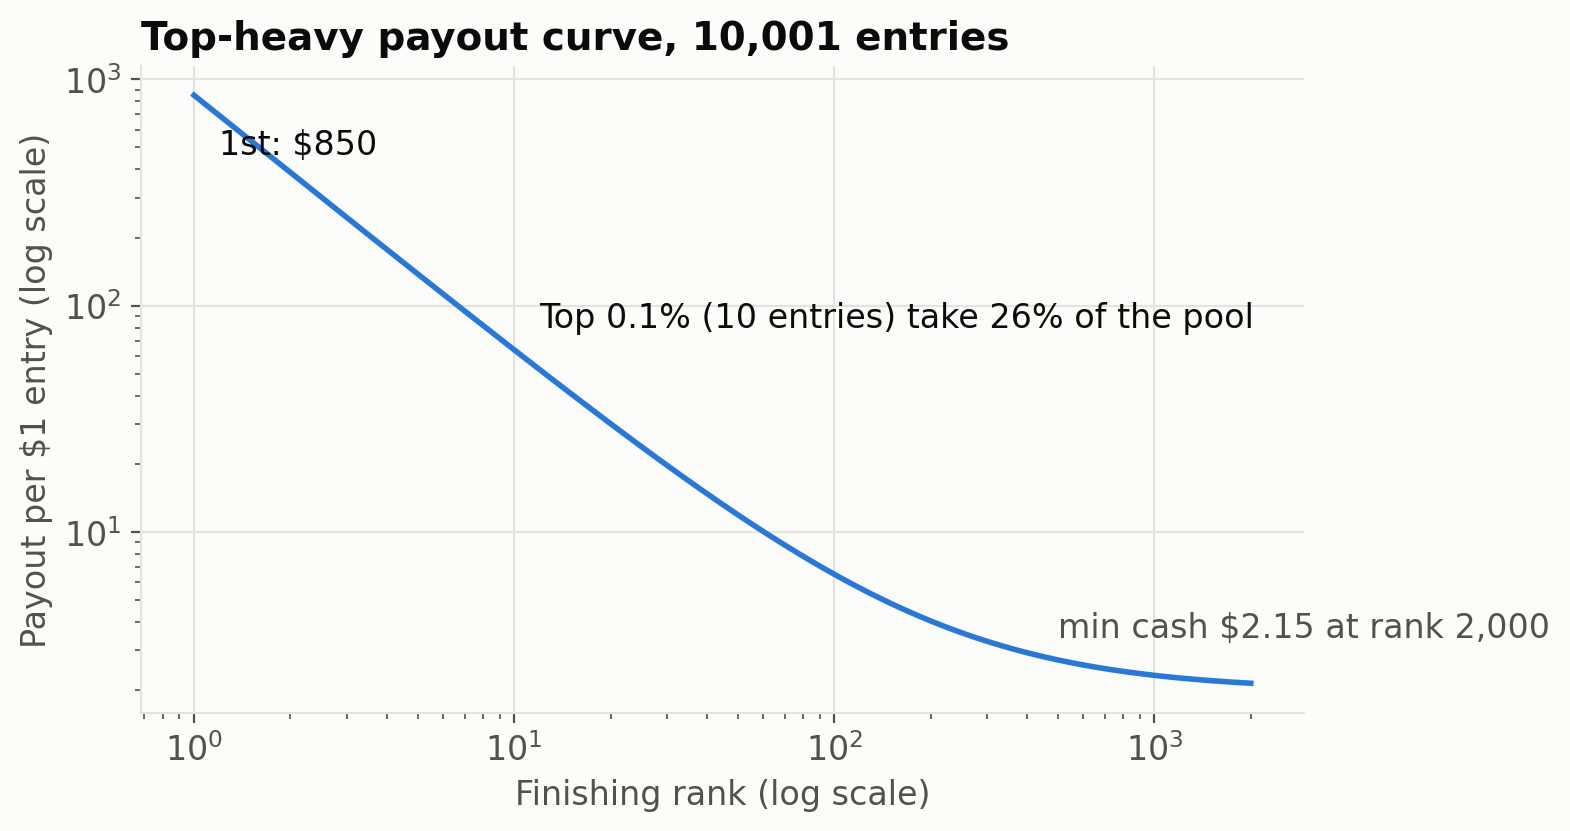
\includegraphics[width=\textwidth]{payout_curve}
    \end{column}
    \begin{column}{0.49\textwidth}
      \centering
      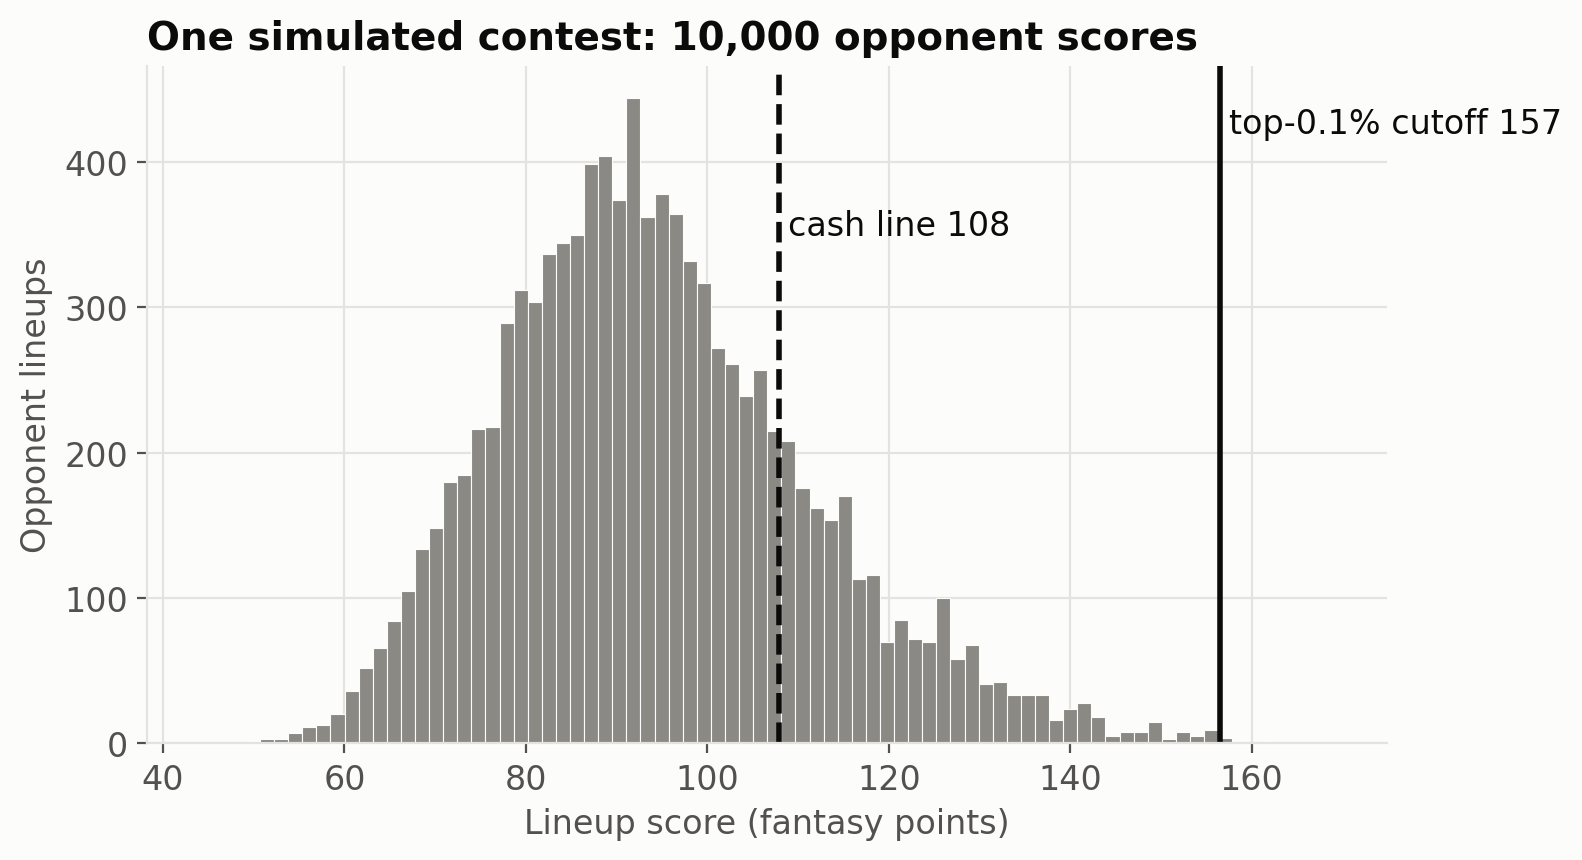
\includegraphics[width=\textwidth]{field_scores}
    \end{column}
  \end{columns}
  \vspace{0.6em}
  \begin{itemize}
    \item Pool $= 0.85 \times 10{,}001$; top 2{,}000 paid: \$2 plus $A\,r^{-g}$, with $g$
      solved so 1st place gets 10\,\% of the pool
    \item Ties (duplicate lineups) split the tied prizes evenly
  \end{itemize}
\end{frame}

\begin{frame}{Backup: importance sampling details}
  \begin{columns}[c]
    \begin{column}{0.49\textwidth}
      \centering
      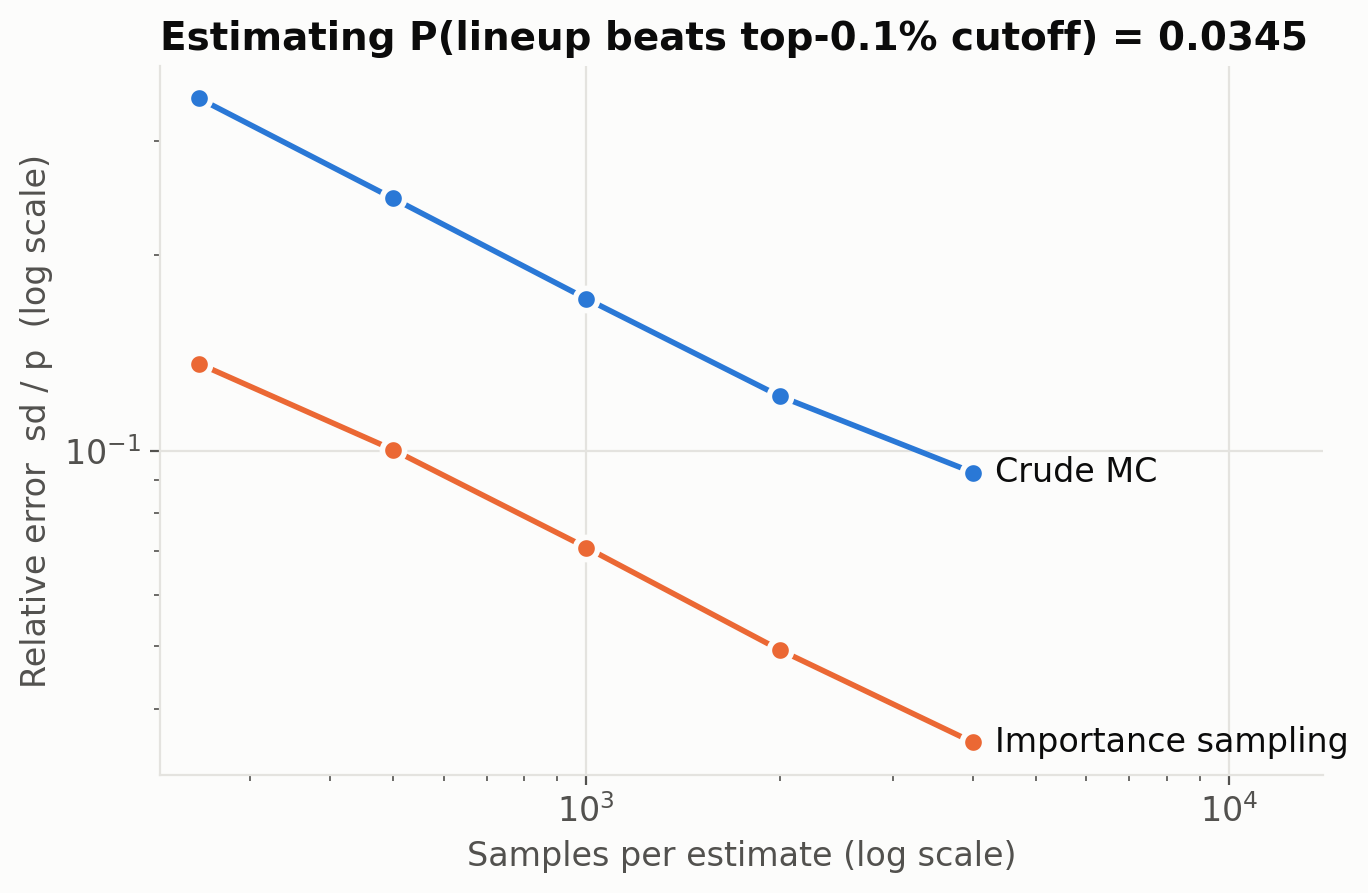
\includegraphics[width=\textwidth]{is_relative_error}
    \end{column}
    \begin{column}{0.49\textwidth}
      \begin{itemize}
        \setlength\itemsep{0.5em}
        \item Score $= \sum_{i \in L} e^{m_i + s_i Z_i}$; gradient at $Z = 0$:
          $a_i = s_i e^{m_i}$ for $i \in L$
        \item Shift the mean along $Ra$: moves the linearized score by $t$ SDs
        \item Pick $t$ by a 20{,}000-draw pilot; $t^* = 1.5$ at the average top-0.1\,\% cutoff
        \item Truth: 2 million crude draws; 300 replications per sample size
      \end{itemize}
    \end{column}
  \end{columns}
\end{frame}

\begin{frame}{Backup: model parameters}
  \centering\small
  \begin{tabular}{@{}ll@{\hspace{2em}}ll@{}}
    \toprule
    Slate & 8 teams, 80 players & Field size $O$ & 10{,}000 \\
    Salary cap $B$ & \$50{,}000 & Sharks & 20\,\% of field \\
    Salary floor $B_{lb}$ & $0.98B$ & Shark noise & 15\,\% (log scale) \\
    Stack probability $q$ & 0.35 & Dirichlet $\kappa$ & 200 \\
    Rake & 15\,\% & Paid places & top 20\,\% \\
    U-CVaR $\alpha$ & 0.99 (S2), 0.975 (S2-CV) & Candidate pool & 323 lineups \\
    Selection & 50 fields $\times$ 100 draws & Test & 200 fields $\times$ 10 draws \\
    \bottomrule
  \end{tabular}
  \vspace{0.8em}

  All defaults are in \texttt{src/dfs/config.py}; separate seeds for generation, selection,
  test and importance sampling.
\end{frame}

\end{document}
